\documentclass[12pt]{article}
\def\activityid{F09-U-v2}\usepackage[letterpaper,margin=.65in,top=.60in,bottom=.65in]{geometry}
\usepackage[T1]{fontenc}
\usepackage[default]{sourcesanspro}
\usepackage{microtype,tikz,array,tabularx,fancyhdr,amsmath,amssymb}
\usepackage[hidelinks]{hyperref}
\usetikzlibrary{calc,arrows.meta}
\setlength{\parindent}{0pt}\setlength{\parskip}{7pt}
\setlength{\headheight}{0pt}\setlength{\footskip}{26pt}\setlength{\emergencystretch}{2em}
\pagestyle{fancy}\fancyhf{}\renewcommand{\headrulewidth}{0pt}\renewcommand{\footrulewidth}{.4pt}
\fancyfoot[L]{\scriptsize Bellingham Math Circle / Week 9 / \activityid}
\fancyfoot[R]{\scriptsize \thepage}
\definecolor{ink}{gray}{.12}\definecolor{soft}{gray}{.95}\color{ink}
\newcommand{\PageTitle}[2]{{\fontsize{10}{12}\selectfont\bfseries WEEK 9\quad BOUNCE LAB\hfill #1\par}\vspace{3pt}{\fontsize{26}{29}\selectfont\bfseries #2\par}\vspace{2pt}}
\newcommand{\NameLine}{{\small Name: \rule{2.65in}{.4pt}\hfill Date: \rule{1.35in}{.4pt}\par}\vspace{4pt}}
\newcommand{\Task}[2]{\par\vspace{3pt}{\large\bfseries #1}\par #2\par}
\newcommand{\Subhead}[1]{\par\vspace{3pt}{\large\bfseries #1}\par}
\newcommand{\RuleBox}[1]{\par\begingroup\setlength{\fboxsep}{8pt}\colorbox{soft}{\parbox{\dimexpr\linewidth-16pt\relax}{#1}}\endgroup\par}
\newcommand{\WriteBox}[2]{\par\textbf{#1}\par\vspace{2pt}\begin{tikzpicture}\draw[black!40,line width=.5pt] (0,0) rectangle (\dimexpr\linewidth-.5pt\relax,#2);\end{tikzpicture}\par}
\newcommand{\StudentFooter}{\vfill{\small Try it with objects. Explain by pointing, talking, or drawing.}\par}
\newcommand{\RookBoard}[3]{\begin{tikzpicture}[x=#3,y=#3]\draw[step=1,black!45] (0,0) grid (#1,#2);\draw[thick] (0,0) rectangle (#1,#2);\node[font=\Large] at ({#1-.5},.5){$\star$};\draw[-{Latex},thick] (0,-.35)--(#1,-.35);\draw[-{Latex},thick] ({#1+.35},#2)--({#1+.35},0);\end{tikzpicture}}
\newcommand{\Table}[3]{\begin{tikzpicture}[x=#3,y=#3]\draw[step=1,black!25] (0,0) grid (#1,#2);\draw[thick] (0,0) rectangle (#1,#2);\fill (0,0)circle(3pt);\draw[-{Latex},very thick] (0,0)--(.7,.7);\node[below] at ({#1/2},-.1){width #1};\node[rotate=90,above] at (-.2,{#2/2}){height #2};\end{tikzpicture}}
\newcommand{\GraphNodes}{\coordinate(A)at(0,0);\coordinate(B)at(3,0);\coordinate(C)at(1.5,2.6);\coordinate(D)at(1.5,.95);}
\newcommand{\Kfour}[1]{\begin{tikzpicture}[scale=#1]\GraphNodes\draw[very thick](A)--(B)--(C)--(A)--(D)--(B) (D)--(C);\foreach \n in {A,B,C,D}{\node[circle,draw,fill=white,minimum size=22pt,font=\bfseries]at(\n){\n};}\end{tikzpicture}}
\newcommand{\House}[1]{\begin{tikzpicture}[scale=#1]\coordinate(A)at(0,0);\coordinate(B)at(3,0);\coordinate(C)at(3,2);\coordinate(D)at(0,2);\coordinate(E)at(1.5,3.3);\draw[very thick](A)--(B)--(C)--(D)--(A) (D)--(E)--(C);\foreach \n in {A,B,C,D,E}{\node[circle,draw,fill=white,minimum size=22pt,font=\bfseries]at(\n){\n};}\end{tikzpicture}}

\begin{document}

\PageTitle{GRADES 4--5}{A straight line in many rooms}\NameLine
\RuleBox{Table sizes are width $w$ by height $h$. Start bottom-left at 45 degrees. Reflect at walls; stop at the FIRST corner. Count a wall bounce, but not the starting or ending corner.}
\Task{1. Trace, then unfold.}{Find the route on a $4\times6$ table. If this trace is familiar, begin with the copied rooms and explain your prediction. Mirror copies let a bounce become a straight continuation. On the copied rooms below, draw the diagonal to the first meeting of a vertical and horizontal room wall.}
\begin{center}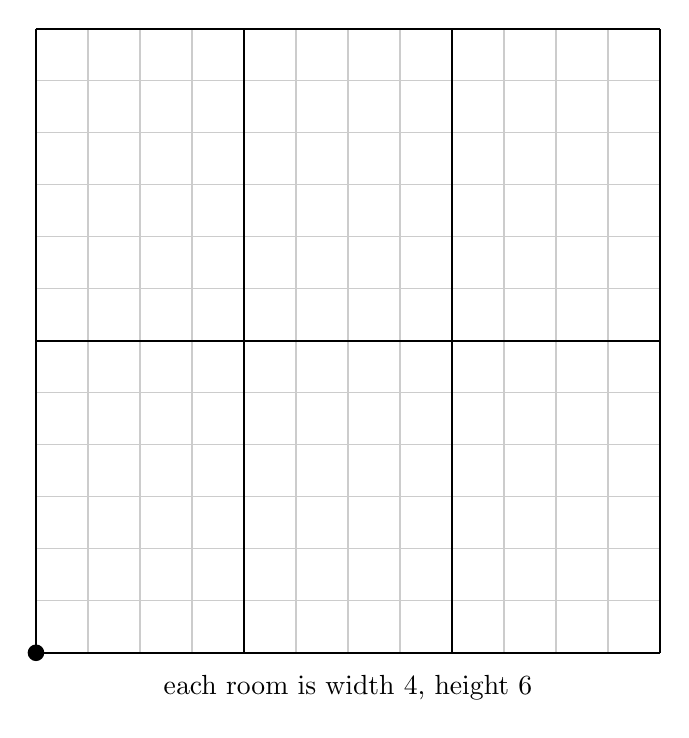
\begin{tikzpicture}[x=.26in,y=.26in]\draw[step=1,black!20](0,0)grid(12,12);\foreach\x in{0,4,8,12}{\draw[thick](\x,0)--(\x,12);}\foreach\y in{0,6,12}{\draw[thick](0,\y)--(12,\y);}\fill(0,0)circle(3pt);\node[below]at(6,-.25){each room is width 4, height 6};\end{tikzpicture}\end{center}
\Task{2. Name the meeting distance.}{Call that horizontal distance $L$. Why must $L$ be a multiple of \emph{both} $w$ and $h$? Why do we take the \emph{least} positive common multiple?}
\WriteBox{Why a corner means a simultaneous wall meeting:}{.85in}
\StudentFooter

\newpage

\PageTitle{GRADES 4--5}{Predict every ending corner}\NameLine
\Task{3. Fold the rooms back.}{If the straight line crosses $m=L/w$ whole room widths, where does it end: right or left? If it crosses $n=L/h$ whole room heights, where does it end: top or bottom?}
\begin{center}\renewcommand{\arraystretch}{1.85}\begin{tabular}{c|c|*{3}{>{\centering\arraybackslash}p{.62in}|}>{\centering\arraybackslash}p{1.1in}}$w$&$h$&$L$&$m$&$n$&Corner\\\hline4&6&&&&\\6&9&&&&\\6&10&&&&\\8&14&&&&\end{tabular}\end{center}
\Task{4. Two even sides: is that enough?}{Compare $4\times6$ with $6\times10$. Both have even side lengths. Why can that rule give the wrong answer?}
\Task{5. A corner too soon.}{Suppose $m,n$ shared a divisor $d>1$. How many whole widths and heights would the path have crossed at distance $L/d$? Why would that already be a corner? Use this to rule out a first ending at bottom-left, which needs both counts even.}
\WriteBox{An earlier corner would mean:}{.55in}
\Task{6. Optional: shrink the side lengths.}{With an adult, write $w=ga,h=gb$, where $g$ is their greatest common divisor. The coprime rule says: if $a,b$ share no factor greater than 1, $b$ divides $at$ only when it divides $t$. For $a=2,b=3$, explain this using $3t-2t=t$. Ask for the general argument. Now $L=ga\,t$ must also be a multiple of $gb$. Why is the least possible $t$ equal to $b$? Conclude $L=gab$, $m=b$, $n=a$.}
\WriteBox{The corner rule in reduced side lengths a and b:}{.55in}
\StudentFooter

\newpage

\PageTitle{GRADES 4--5}{How many bounces is best?}\NameLine
\Task{7. Count walls instead of drawing.}{Before the final corner, how many vertical room walls does the unfolded line cross? How many horizontal room walls? Could a meeting be counted twice before the first corner?}
\WriteBox{A formula in m,n (or a,b after task 6), with a reason:}{1.0in}
\Task{8. Optional proof continuation: inverse design.}{Design a whole-number rectangle ending at the \textbf{top-right after exactly four bounces}. Find all the possible reduced width/height pairs. Then make a second size with the same shape.}
\WriteBox{All reduced pairs, and why there are no others:}{1.05in}
\Task{9. An impossible order?}{An adult requests a table ending at the top-right after exactly \textbf{three} bounces. Find one, or prove it cannot exist.}
\WriteBox{My construction or obstruction:}{.95in}
\textbf{Researcher's habit:} Distinguish a table you failed to find from a table you can prove does not exist.
\StudentFooter

\end{document}
